\documentclass[pdftex,11pt,letterpaper]{article}
\usepackage{indentfirst}
\usepackage[titletoc]{appendix}% http://ctan.org/pkg/appendices
\usepackage{fullpage}
\usepackage{listings}
\usepackage{color}
\usepackage{float}
\usepackage{amsmath}

\restylefloat{figure}


\definecolor{dkgreen}{rgb}{0,0.6,0}
\definecolor{gray}{rgb}{0.5,0.5,0.5}
\definecolor{mauve}{rgb}{0.58,0,0.82}
 
\lstset{ %
  language=Python,                % the language of the code
  basicstyle=\footnotesize,           % the size of the fonts that are used for the code
  numbers=left,                   % where to put the line-numbers
  numberstyle=\tiny\color{gray},  % the style that is used for the line-numbers
  stepnumber=1,                   % the step between two line-numbers. If it's 1, each line 
                                  % will be numbered
  numbersep=5pt,                  % how far the line-numbers are from the code
  backgroundcolor=\color{white},      % choose the background color. You must add \usepackage{color}
  showspaces=false,               % show spaces addisng particular underscores
  showstringspaces=false,         % underline spaces within strings
  showtabs=false,                 % show tabs within strings adding particular underscores
  frame=single,                   % adds a frame around the code
  rulecolor=\color{black},        % if not set, the frame-color may be changed on line-breaks within not-black text (e.g. comments (green here))
  tabsize=2,                      % sets default tabsize to 2 spaces
  captionpos=b,                   % sets the caption-position to bottom
  breaklines=true,                % sets automatic line breaking
  breakatwhitespace=false,        % sets if automatic breaks should only happen at whitespace
% title=\lstname,                   % show the filename of files included with \lstinputlisting;
                                  % also try caption instead of title
  keywordstyle=\color{blue},          % keyword style
  commentstyle=\color{dkgreen},       % comment style
  stringstyle=\color{mauve},         % string literal style
  escapeinside={\%*}{*)},            % if you want to add a comment within your code
  morekeywords={*,...}               % if you want to add more keywords to the set
}

\definecolor{maroon}{rgb}{0.5,0,0}
\definecolor{darkgreen}{rgb}{0,0.5,0}
\lstdefinelanguage{XML}
{
  basicstyle=\ttfamily,
  morestring=[s]{"}{"},
  morecomment=[s]{?}{?},
  morecomment=[s]{!--}{--},
  commentstyle=\color{darkgreen},
  moredelim=[s][\color{black}]{>}{<},
  moredelim=[s][\color{red}]{\ }{=},
  stringstyle=\color{blue},
  keywordstyle=\color{blue},          % keyword style
  commentstyle=\color{dkgreen},       % comment style
  stringstyle=\color{mauve},         % string literal style
}

\newcommand{\HRule}{\rule{\linewidth}{0.5mm}}

% Added by Stokes
\usepackage{datenumber}
\usepackage{tabto}
\setlength\parindent{0pt}
\usepackage{fancyhdr}
\usepackage{lastpage}
\usepackage{multirow}
\usepackage[table]{xcolor}% http://ctan.org/pkg/xcolor
\pagestyle{fancy}
\usepackage{tikz} % rounded corners
\usepackage{array}
\usepackage{amssymb}
\usepackage[colorlinks=false, pdfborder={0 0 0}]{hyperref}
\usepackage{url}  % This makes \url works

% set table column width
\newcolumntype{L}[1]{>{\raggedright\let\newline\\\arraybackslash\hspace{0pt}}m{#1}}
\newcolumntype{R}[1]{>{\raggedleft\let\newline\\\arraybackslash\hspace{0pt}}m{#1}}
% box
\newcommand{\mybox}{\mbox{\ooalign{\cr\hidewidth$\square$\hidewidth\cr}}}
% Footer
\fancyhf{}
\renewcommand{\headrulewidth}{0pt}
\fancyfoot[C]{\textit{\textbf{Matthew Stokes\\}}Page \thepage\ of \pageref{LastPage}}

\usepackage{appendix}

% subsubsubsection
\usepackage{titlesec}
\setcounter{secnumdepth}{4}
\titleformat{\paragraph}
{\normalfont\normalsize\bfseries}{\theparagraph}{1em}{}
\titlespacing*{\paragraph}
{0pt}{3.25ex plus 1ex minus .2ex}{1.5ex plus .2ex}
\newcommand{\ihat}{\boldsymbol{\hat{\textbf{i}}}}
\newcommand{\jhat}{\boldsymbol{\hat{\textbf{j}}}}
\newcommand{\khat}{\boldsymbol{\hat{\textbf{k}}}}
\begin{document}

\begin{titlepage}

\begin{center}

\HRule \\[0.4cm]
{ \huge \bfseries Force-Displacement Glenoid Reamer Guide}\\[0.4cm]

\HRule \\[1.5cm]

% Upper part of the page
\begin{center}

\includegraphics[width=0.4\textwidth]{./images/jo.png}\\[1cm]  
\hspace{2cm}
\includegraphics[width=0.7\textwidth]{./images/icon.png}\\[1cm]

\includegraphics[width=0.6\textwidth]{./images/hulc.jpg}\\[1cm] 
\end{center}


% Title

\vspace{4cm}
% Author and supervisor
\begin{minipage}{0.4\textwidth}
\begin{flushleft} \large
\emph{Author:}\\
\textsc{Matthew Stokes}
\end{flushleft}
\end{minipage}
\begin{minipage}{0.4\textwidth}
\begin{flushright} \large
\emph{} \\
\textsc{}
\end{flushright}
\end{minipage}


\vfill
% Bottom of the page
{\today}

\end{center}

\end{titlepage}
\pagebreak
\tableofcontents
\thispagestyle{fancy}
\pagebreak
\listoffigures
\thispagestyle{fancy}
\pagebreak
\listoftables
\thispagestyle{fancy}
\pagebreak


%\setcounter{page}{1}
\section{Overview} 
Reamer project was designed to calculate the applied force and resulting displacement of the glenoid during reaming. However due to modern sensor limitations (namely a small wireless load cell) the reamer will not be rotating during measurements. \\

This document includes information pertaining to setting up the system, recording measurements from the sensors, and interacting with this information. It does not include any background information about the project.

\section{Equipment}
Equipment has been separated into six distinctly different categories: sensing and tools, 3D printed attachment parts, DAQ \& other intermediary electronics, software, supplementary files, and misc. 


\subsection{Sensing and Tools}

\begin{table}[h!]
\begin{center}
    \begin{tabular}{ | c | l | l | l |}
    \hline
    Item & Product & Manufacture & Description \\ \hline
    1 & Load cell & ATI & Nano25 FT 13036 \\ \hline  
    2 & Optotrack Certus & NDI & Optical Camera \\ \hline
    3 & Optical tracker & NDI & \\ \hline
    4 & Reamer & & Surgical reamer \\ \hline
    \end{tabular}
    \caption{Sensing and Tools}
\end{center}
\end{table}

\subsection{3D Printed Attachment Parts}
All parts were designed by Matthew Stokes and printed on his MakerBot Replicator using the settings 100\% infill, 0.2mm layer height. 

\begin{table}[h!]
\begin{center}
    \begin{tabular}{ | c | l | l |}
    \hline
    Item & Product & Description \\ \hline
    5 & Head Couple & Between head of reamer and load cell \\ \hline  
    6 & Back Plate Couple & Between back plate of load cell and reamer shaft \\ \hline
    7 & Reamer Attachment Plate & Base connecting to the reamer \\ \hline
    8 & Optical Tracker Attachment Plate & connecting to the reamer attachment plate \\ \hline
    9 & Standoff & Hidden via thru hole securing reamer attachment plate \\ \hline  
    \end{tabular}
    \caption{3D Printed Attachment Parts}
\end{center}
\end{table}

\pagebreak
\subsection{DAQ \& Other Intermediary Electronics}
Necessary intermediary products connecting to sensors and involved in setup/calibration. 
\begin{table}[h!]
\begin{center}
    \begin{tabular}{ | c | l | l | l |}
    \hline
    Item & Product & Manufacture & Description \\ \hline
    10 & Wireless Strober & NDI & Strobe the optical trackers \\ \hline
    11 & Stylist & NDI & tracker offset to tip of stylist \\ \hline
    12 & Optotrak Box & NDI & Sync strober and tracking camera \\ \hline
    13 & Load Cell DAQ & ATI & filter and amplify \\ \hline
    14 & Multifunction DAQ & NI & load cell DAQ to USB  \\ \hline
    15 & Computer & & Windows XP \\ \hline
	\end{tabular}
	\caption{DAQ \& Other Intermediary Electronics}
\end{center}
\end{table}

\subsection{Software}

\begin{table}[h!]
\begin{center}
    \begin{tabular}{ | c | l | l | l |}
    \hline
    Item & Program & Author & Description \\ \hline
    16 & Motion Station & HULC Lab & LabView optical tracker measurements \\ \hline
    17 & Loadcelly & Stokes & LabView load cell measurements \\ \hline
    18 & pushpush.py & Stokes & Python interacting with data output \\ \hline
    19 & ATIDAQFT.NET & ATI & Native software \\ \hline
    20 & NDI First Principals & NDI & Native software \\ \hline
    21 & NI Measurement \& Automation & NI & Native software \\ \hline
	\end{tabular}
	\caption{Software}
\end{center}
\end{table}

\subsection{Supplementary Software Files}
These files should not be modified. 
\begin{table}[h!]
\begin{center}
    \begin{tabular}{ | c | l | l | l |}
    \hline
    Item & File Name & Extension & Description \\ \hline
    22 & nano25calibration & .cal & load cell calibration \\ \hline
    23 & bsty0213 & .rig & rigid body for the stylist \\ \hline
    24 & smart\_02 & .rig & rigid body for base NI optical tracker \\ \hline
	\end{tabular}
	\caption{Supplementary Software Files}
\end{center}
\end{table}

\pagebreak
\subsection{Misc Cables, Nuts, Bolts, Wires}

\begin{table}[h!]
\begin{center}
    \begin{tabular}{ | c | l | l |}
    \hline
    Item & Product &  Description \\ \hline
    25 & Threaded Rob & Connecting head couple to load cell \\ \hline
    26 & 4x Bolts & Connecting reamer attachment plate and optical tracker plate \\ \hline
    27 & 4x Nuts & \\ \hline
    28 & 2x Screws & Attach reamer attachment plate to standoff \\ \hline
    29 & Broken out 24 Pin Cable & Connect Load Cell DAQ to NI-USB-6211 \\ \hline
    30 & Thread & Secure reamer attachment plate to back end of reamer \\ \hline
	\end{tabular}
	\caption{Misc Cables, Nuts, Bolts, Wires}
\end{center}
\end{table}

\section{Hardware Setup}
The project consists of two main systems which are the load cell and the optical tracker. Setup for each of these systems is independent. The reamer itself will be setup as shown in the image below. \\

\begin{figure}[ht!]
\centering
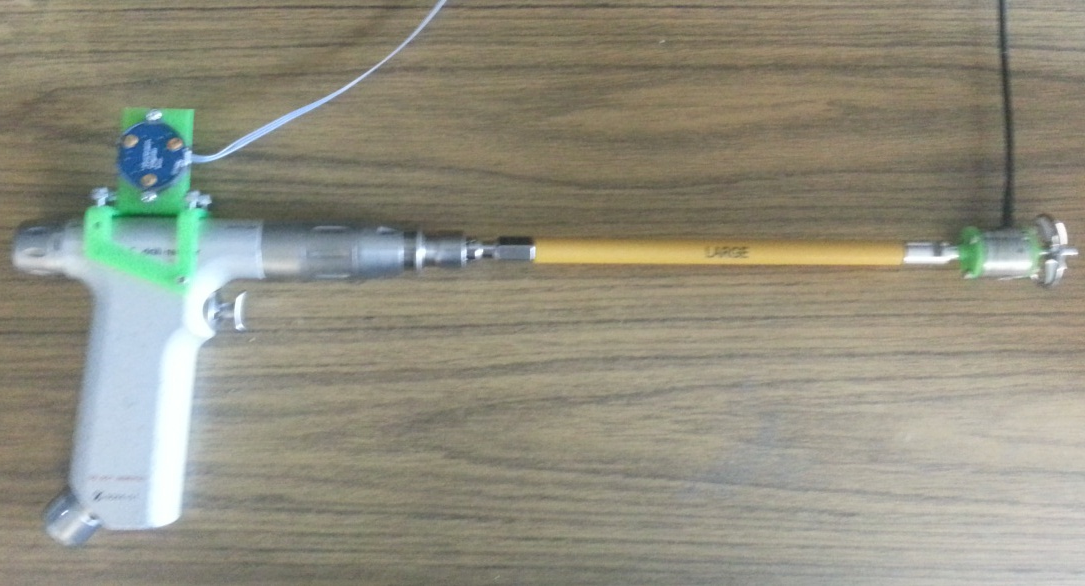
\includegraphics[width=100mm]{./images/reamer_total}
\caption{Reamer Outfitted with Load Cell and Optical Tracker}
\label{reamer}
\end{figure}

Contained in this assembly are the following items: \\
\pagebreak
\begin{table}[h!]
\begin{center}
    \begin{tabular}{ | c | l |}
    \hline
    Item & Product \\ \hline
    1 & Load Cell \\ \hline
    3 & Optical Tracker \\ \hline
    4 & Reamer \\ \hline
    5 & Head Couple \\ \hline
    6 & Back Plate Couple \\ \hline
    7 & Reamer Attachment Plate \\ \hline
    8 & Optical Tracker Plate \\ \hline
    9 & Standoff \\ \hline
    25 & Threaded Rod \\ \hline
    26 & 4X Bolts \\ \hline
    27 & 4X Nuts \\ \hline
    28 & 2X Screws \\ \hline
    30 & Thread \\ \hline
	\end{tabular}
	\caption{Reamer Assembly Parts List}
\end{center}
\end{table}

\subsection{Optical System Setup}
An overview of the optical system setup is shown in the image below. \\

\begin{figure}[ht!]
\centering
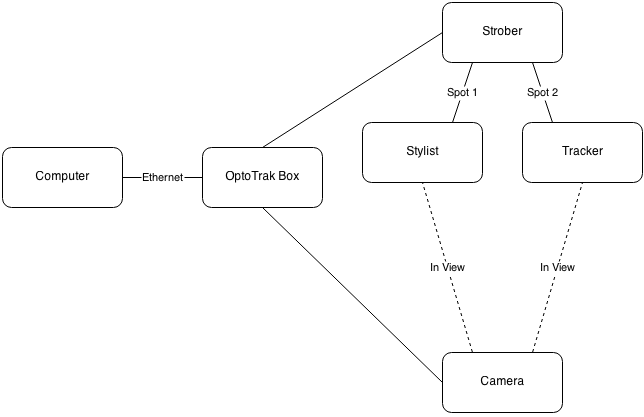
\includegraphics[width=150mm]{./images/ot_overview}
\caption{Optical Tracker System Overview}
\end{figure}

Plugin and power on the optical tracker camera. You should see a green light which indicates the power is on. The optical tracker camera communicates with the Optotrak Box which is connected via Ethernet to the main computer. Power on the Optotrak Box and plug the cable into the optical tracker. \\

\begin{figure}[ht!]
\centering
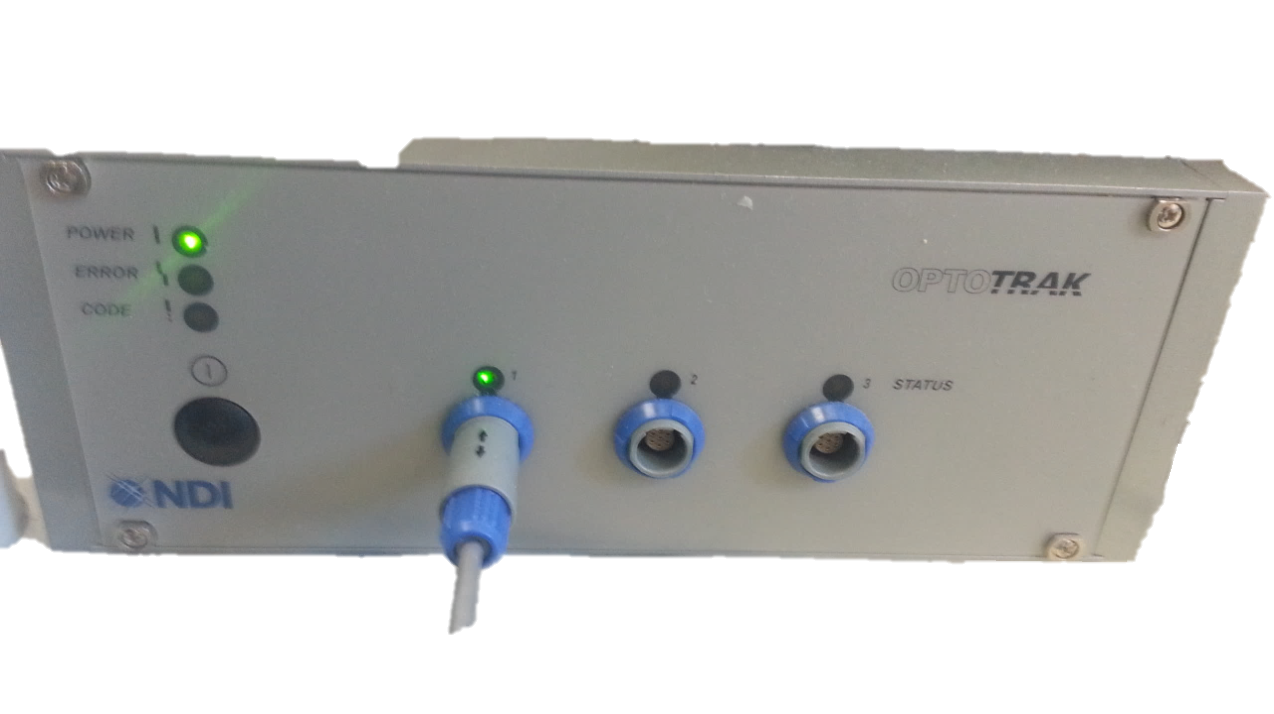
\includegraphics[width=120mm]{./images/optotrak_box}
\caption{Optotrak Box}
\end{figure}

\begin{figure}[ht!]
\centering
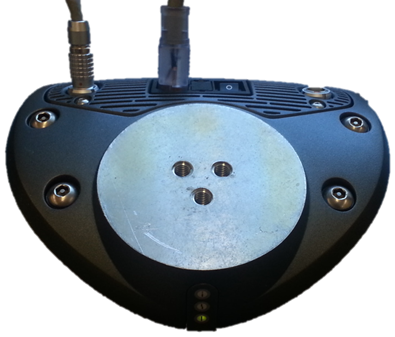
\includegraphics[width=80mm]{./images/ot_camera}
\caption{Certus Optical Camera}
\end{figure}

Next we need to wire the tracker on our reamer. The tracker should connect to the strober box which can hold up to 5 trackers. Trackers may also be daisy chained with up to 4 trackers. To begin we will wire the tracker as part of our reamer assembly and also a stylist (which we be used for offset calibration). Note we will wire the stylist in port 1 and the tracker in port 2. This order matters later. \\

\subsubsection{Setup Test}
To ensure the system is setup properly open NDI First Principals and click \textit{Create New} \\

\begin{figure}[ht!]
\centering
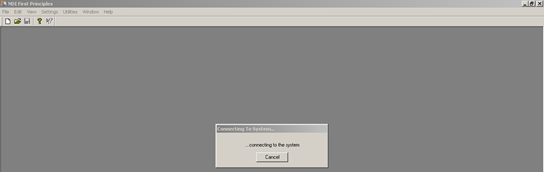
\includegraphics[width=150mm]{./images/ot}
\caption{NDI First Principals}
\end{figure}

If everything is connected we should will be taken to the next screen for setting up a new project seen below. Else go back and try again. \\

\begin{figure}[ht!]
\centering
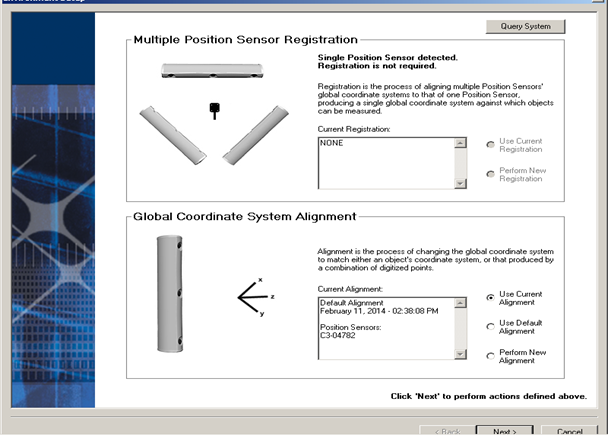
\includegraphics[width=150mm]{./images/ot_2}
\caption{NDI First Principals}
\end{figure}

\subsubsection{Offset Calibration}
Now that we know our optical tracker is being read by the camera we will calculate the offset between the center of the tracker and the tip of the reamer. We do because we are interested in the displacement of the tip as opposed to the displacement of the tracker. This allows us to also pivot about the tip without measuring any displacement. \\

To determine the offset we will position the stylist to touch the tip of the reamer and record the x,y,z values of both the stylist and the other tracker. The difference between these values will be our offset. We will later offset the trackers calibration matrix by these values in return to motion station. \\

Clicking the \textit{Next} button on the multiple position sensor registration screen should take us to the experiment setup screen shown below.\\

\begin{figure}[ht!]
\centering
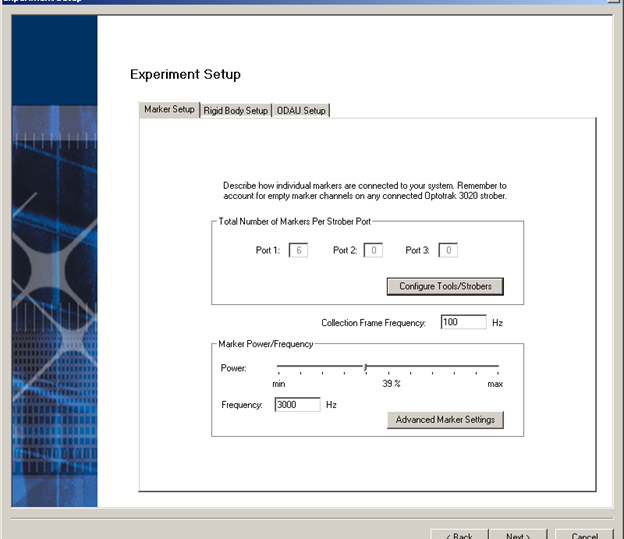
\includegraphics[width=150mm]{./images/exper_setup}
\caption{Experiment Setup}
\end{figure}

Here we should see \textbf{6 total markers}- 3 from our stylist and 3 from our tracker. If you do not see six total then something has not been setup correctly. \\

At this stage we are required to modify some of the settings in order to get better functionality out of our optical system. Modify the following parameters: 

\begin{table}[h!]
\begin{center}
\begin{tabular}{l*{1}{r}}
Parameter             & New Value \\
\hline
Collection Frame Frequency & 50   \\
Frequency & 3500   \\
Advanced | Duty Cycle & 80   \\
\end{tabular}
	\caption{Reamer Assembly Parts List}
\end{center}
\end{table}

These modifications are also shown in the images below. \\

\begin{figure}[ht!]
\centering
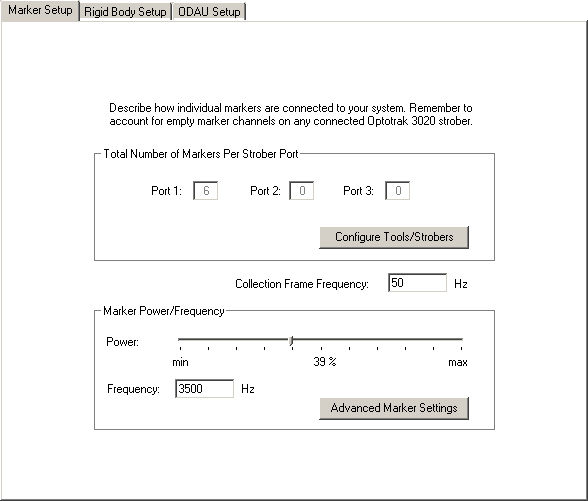
\includegraphics[width=130mm]{./images/marker_setup}
\caption{Marker Setup}
\end{figure}

\begin{figure}[ht!]
\centering
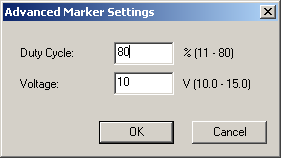
\includegraphics[width=60mm]{./images/adv_marker_setup}
\caption{Advanced Marker Settings}
\end{figure}

Once these settings have been changed we need to click on the Rigid Body Setup Tab. \\

\begin{figure}[ht!]
\centering
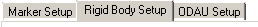
\includegraphics[width=50mm]{./images/tab}
\caption{Rigid Body Setup Tab}
\end{figure}

Here we need to add two rigid body files which can be found in Appendix A: \textbf{bsty0213.rig} and \textbf{smart\_02.rig}. Bsty2013 was created in house and smart\_02 is the rigid body file for a tracker created by NDI. These files contain information used by the camera to interoperate 3 markers as a rigid body. You must ensure to load the bsty0213 file before the smart\_02 file as this is order corresponds to our placement earlier. The completed rigid body setup is shown below. 

\begin{figure}[ht!]
\centering
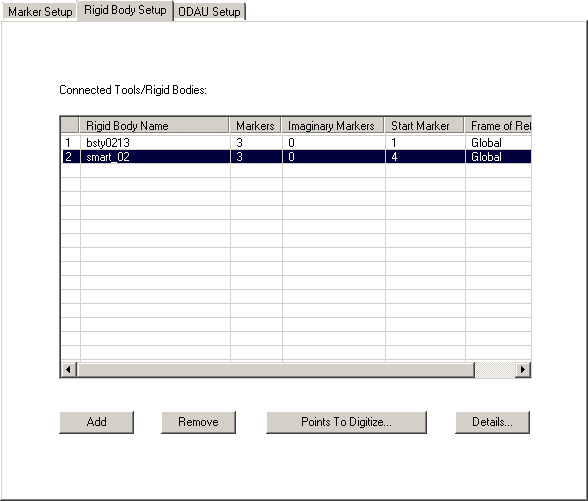
\includegraphics[width=150mm]{./images/ridges}
\caption{Two Rigid Bodies}
\end{figure}

We can now click \textit{Next} as we are finished the experimental setup. Clicking \textit{Next} may or may not prompt you with the screen seen below. Click \textit{no}. Just do it. You are lying to yourself if you believe this will actually work in wireless mode.  

\begin{figure}[ht!]
\centering
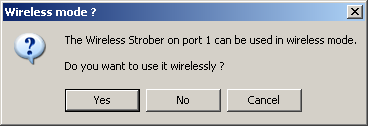
\includegraphics[width=65mm]{./images/wireless}
\caption{Wireless Mode}
\end{figure}

Green means the camera can see the markets and I assume you can figure out what red means. Interesting note: if you are in an odd situation where you think it should be reading values but it's not simply put you hand in front of the tracker to hide it from the camera then remove it. This does something along some lines of “resetting” some internal stuff. \\

Click the \textit{View} | \textit{Probe View}. This should present you with a screen similar to the one shown below (minus any actual values…we`re getting there). 

\begin{figure}[ht!]
\centering
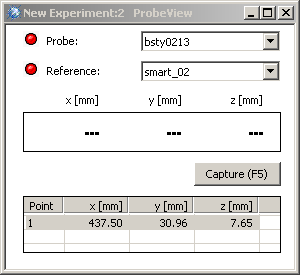
\includegraphics[width=65mm]{./images/offset}
\caption{Offset}
\end{figure}

This is where we determine the offset. We use the smart\_02 sensor as the reference and the bsty0213 as the probe. Then once both rigid bodies are green (in sight) it should start showing values which are the difference between the two trackers. It`s important to note that the stylist has already been configured to offset its tracker to the tip so measurements are from the tip of the stylist to the center of the optical tracker on the reamer. \\

Touch the tip of the stylist to the tip of the reamer and hit \textit{F5} or the \textit{Capture} button. The resulting values should be similar to the ones shown in the image above else something has really changed which is odd. Record these values somewhere as we will use these soon. 
It`s at this time we are ready to move on to using Return of the Motion Station (yay). But before we do this we will take a second to setup our load cell. 

\subsection{Load Cell Setup}
An overview of the optical system setup is shown in the image below. \\

\begin{figure}[ht!]
\centering
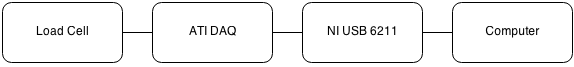
\includegraphics[width=150mm]{./images/lc_overview}
\caption{Load Cell Overview}
\end{figure}


The load cell plugs into the ATI DAQ box. This box connects to the NI USB-6211 device via a special broken out cable. \\


\begin{figure}[ht!]
\centering
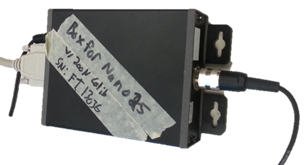
\includegraphics[width=100mm]{./images/nano25}
\caption{ATI DAQ}
\end{figure}

\begin{figure}[ht!]
\centering
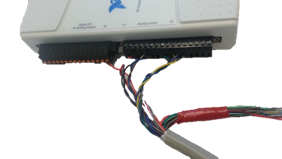
\includegraphics[width=100mm]{./images/broke}
\caption{Broken 24 Pin Cable}
\end{figure}

Finally, the NI USB-6211 box connects to the USB port on the main computer.

\begin{figure}[ht!]
\centering
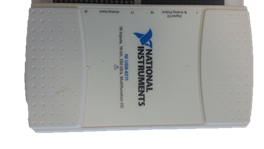
\includegraphics[width=70mm]{./images/usb}
\caption{NI USB-6211}
\end{figure}

\subsubsection{Setup Test}
Open NI Measurement \& Automation Explorer which should display the screen shown below.\\

\begin{figure}[ht!]
\centering
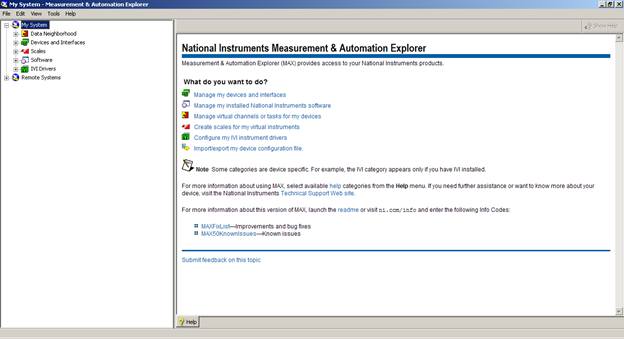
\includegraphics[width=150mm]{./images/ni_ma}
\caption{National Instruments Measurement \& Automation Explorer}
\end{figure}

Select \textit{Devices and Interfaces} | \textit{NI-DAQmx Devices} and make note of the \textbf{DEV port} for NI USB-6211 (in our example its DEV 4 but yours may differ). \\ 

\begin{figure}[ht!]
\centering
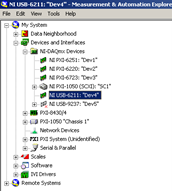
\includegraphics[width=50mm]{./images/dev4}
\caption{DEV port}
\end{figure}

\pagebreak

Next open ATIDAQFT.NET program shown below. 

\begin{figure}[h!]
\centering
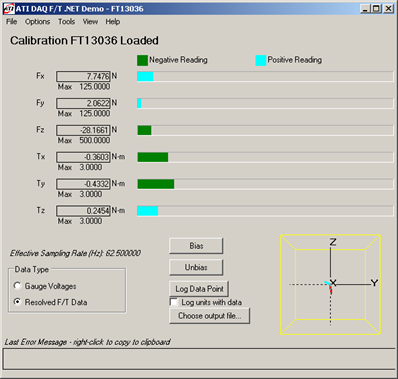
\includegraphics[width=80mm]{./images/cal}
\caption{ATIDAQFT.NET}
\end{figure}

If the load cell values shown on this screen won’t stop climbing than you haven’t selected the proper DEV port for viewing. To change DEV ports click \textit{Options} | \textit{DAQ Hardware Options} shown below and change the device name to your DEV port. Also important to note is that our load cell works over channels 0-5 (X, Y, Z force and Rx, Ry, Rz torques). \\

\begin{figure}[ht!]
\centering
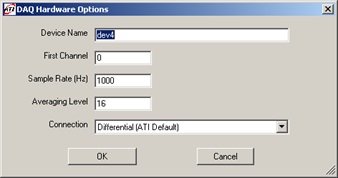
\includegraphics[width=70mm]{./images/dev_p}
\caption{DAQ Hardware Options}
\end{figure}

Click \textit{Ok} and now you should see your load cell values as shown previously. If not you have configured something wrong and you need to go back and fix this. \\

At this stage we have both our load cell and optical tracker setup properly and we are now ready to move on and get acquainted with our software systems for recording sensor measurements and parsing the data.  


\section{Sensor Software}

You have already been exposed to the native software for the load cell and optical tracker and used these native solutions to ensure our hardware is configured properly. Along with the setup software we have used thus far we will also be using three main pieces of software: return to the motion station- to record optical tracker values, loadcelly- to record load cell values, and pushpush.py to parse all the data super easily. \\

\subsection{Return of the Motion Station}
Return to motion station which was developed origionally by Dr. Ferreira as part of his PhD simulator and since then has been expanded by a number of coop students. It enjoys crashing and freezing all the time but there really is no better alternative and as buggy as it is, still provides much added value. \\

Start by opening Return of the Motion Station. You may notice that one of the main windows doesn’t enjoy life, that’s fine just ignore it. 

\begin{figure}[ht!]
\centering
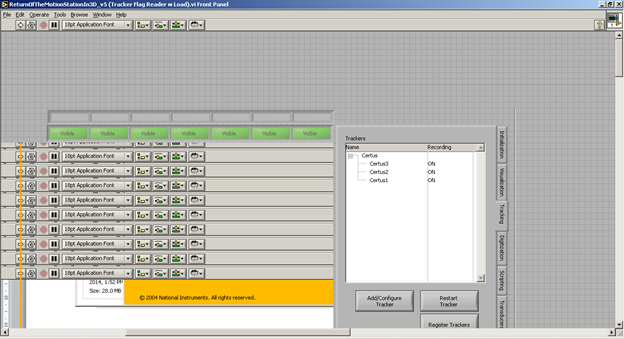
\includegraphics[width=100mm]{./images/rtms}
\caption{Return to the Motion Station}
\end{figure}

\textit{Run} the project and you should be prompted with the screen shown below.

\begin{figure}[ht!]
\centering
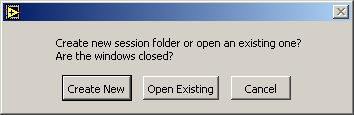
\includegraphics[width=60mm]{./images/create_new}
\caption{Create New Session Folder}
\end{figure}

Since this is our first time running the program we should Create New however once you have already setup the experiment you can just open your already existing session folder. \\

Creating a new session should make the large window go black and pretty much nothing else visible will happen. (It will create all the folders structure behind the scenes among other things). 

\begin{figure}[ht!]
\centering
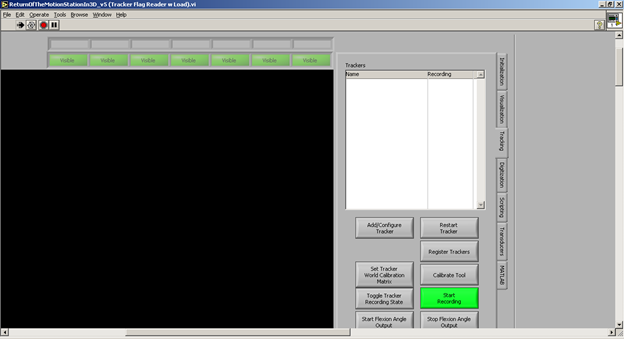
\includegraphics[width=150mm]{./images/rtms2}
\caption{Return to Motion Station Running}
\end{figure}

Now we want to add our optical tracker. At this point if we haven’t already we can remove the stylist as we should only have the optical tracker attached to our reamer in slot 1 of our strober. I will repeat. We should only have 1 optical tracker plugged into strobber in slot 1 which is the tracker attached to the reamer. \\

Click \textit{Add/Configure Tracker} which will display the window shown below. We will select the \textit{Certus} option as we are using a Certus tracker

\begin{figure}[ht!]
\centering
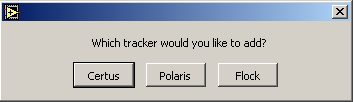
\includegraphics[width=70mm]{./images/flock}
\caption{Add/Configure Tracker}
\end{figure}

Selecting Certus will bring up the Certus Setup Dialog.vi shown below

\begin{figure}[ht!]
\centering
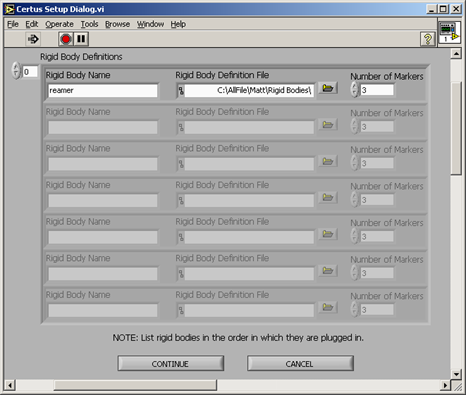
\includegraphics[width=120mm]{./images/certus_setup}
\caption{Certus Setup}
\end{figure}

Here we want to add our smart\_02 rigid body and we can name it whatever we like. This is shown in the image above. Click \textit{Continue}. \\

At this stage we should be brought back to the main screen and the certus optotrak box should start beeping at us. Give this process about 2-3 minutes. Don’t touch anything Motion Station is really sensitive right now. Once the process is done we should see the first slot either turn green or red which means we’ve successfully added our optical tracker into Motion Station. \\

Next we need to tell motion station to record the tracker. This is easily done with selecting the Certus 1 tracker from the list of trackers and clicking T\textit{oggle Tracker Recording State}. This should add \textit{ON} to the list of trackers column. \\

The last thing we must do is \textit{Calibrate Tool} to add the offset we calculated earlier. Click \textit{Calibrate Tool} to bring up the \textit{Calibration Dialog.vi}. Insert the values you recorded into the far right column of the matrix and inset 1’s along the diagonal. This is shown below.

\begin{figure}[ht!]
\centering
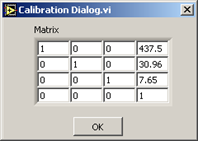
\includegraphics[width=60mm]{./images/cal_mat}
\caption{Calibration Matrix}
\end{figure}

To ensure our calibration matrix has been set, after clicking \textit{OK} scroll down and look for the vi \textit{Tool Calibrated Offsets} as shown in the image below. If these values aren’t the same as the matrix you just inputted you’ve done something wrong. \\

Wonderful! Now we are all ready to being recording. To do this as you may have guessed click the big green Start Recording button and once we stop recording we will be prompted to enter a filename. But first before we get underway with our experiment we need to configure our load cell to a state where it too is ready to record on the press of a button. 

\subsection{Loadcelly}

Loadcelly was designed to read input voltages from a load cell on a given DEV, run these through a calibration script (given by ATI), and output values in N to screen with the ability to record these values to a file. General program can be seen below. This is the program you will use to get load cell values. \\

\begin{figure}[ht!]
\centering
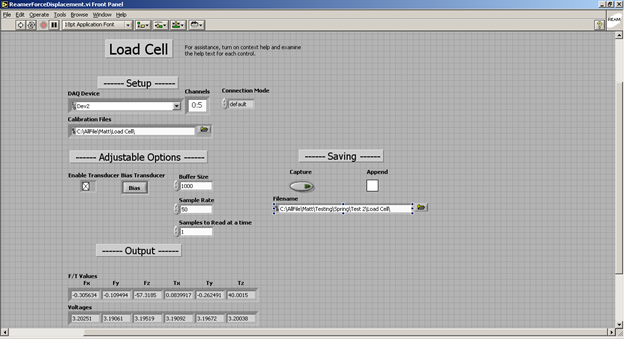
\includegraphics[width=150mm]{./images/celly}
\caption{Loadcelly}
\end{figure}

To use this program first we must select the DEV which our load cell is on. If you don’t know what DEV port this is on refer back to the step where we find the NI-6211 DEV. \\

Next we must load our calibration script (supplied by ATI). If you don’t have this calibration script it is included as Appendix A.  

\begin{figure}[ht!]
\centering
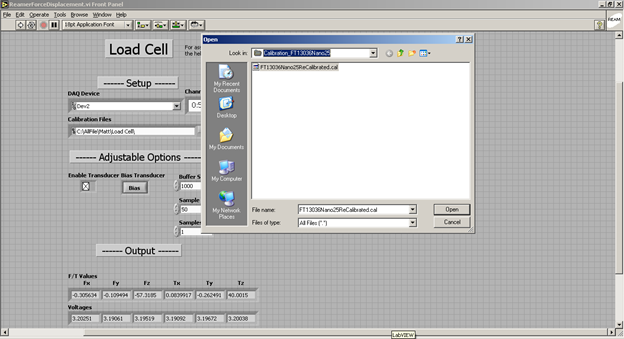
\includegraphics[width=150mm]{./images/celly_2}
\caption{Loadcelly Calibration File}
\end{figure}

Run the program! You should see the force and voltage values constantly jump which means yay you’re reading the load cell sensor values in the program. \\

An option worth mentioning is the BIAS button which will bias the load cell values. You can press this if you like but my later awesome software program will handle this if you don’t. \\
 
Lastly when you are ready to record you should first name the file and select a location then hit the Capture button which will turn green and start recording. \\

\subsection{Recording}

Recording is easy. Click the record button in each of the two programs then go preform your experiment. Once the experiment is done stop both recordings (motion station will prompt you to save the motion record and the file will be in XXX location) \\

\begin{figure}[ht!]
\centering
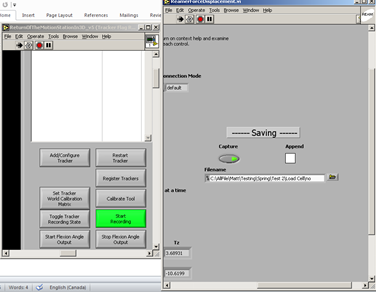
\includegraphics[width=150mm]{./images/record}
\caption{Recording}
\end{figure}

The optical tracker file is outputted with the following headers:

\begin{table}[h!]
\begin{center}
    \begin{tabular}{ | l | l | l | l |}
    \hline
    Timestamp & Dx & Dy & Dz \\ \hline
	\end{tabular}
	\caption{ot.csv}
\end{center}
\end{table}

The load cell file is outputted with the following headers:

\begin{table}[h!]
\begin{center}
    \begin{tabular}{ | l | l | l | l |}
    \hline
    Timestamp & Fx & Fy & Fz \\ \hline
	\end{tabular}
	\caption{lc.csv}
\end{center}
\end{table}

The programs can be combined but greater minds than mine are needed to do this inside of Motion Station. So instead you will have the two programs run simultaneously and you will output two text files which will then be imported into the program pushpush.py which will do many awesome things including automatically trimming the data to remove wait times before or after recording, bias, normalize, filter, and export ready to be plotted. 

\section{Experimental Procedure}
We are looking to measure values from a push. You may record as many pushes as you like however it is recommended that you add a pause > 0.25s between each push so that the events can be considered independent.

\section{Post Processing}
Pushpush.py is used to extract raw information from the two text files and allow the user access to this in a much more manageable form (Motion Station outputs irrelevant information for our experiment, in a non-consistent formatting). Pushpush.py utilizes abstraction, inheritance, and the visitor design pattern to provide us easy access to our sensor data. \\

The main.py file is your main interaction with the program. The program should be called in the following manner and requires 3 command line arguments:

\begin{lstlisting}
python main.py –lc inputfilepath –ot inputfilepath –o outputfilepath
\end{lstlisting}

The output file path will be created if it does not already exist. The program will not execute if improper arguments have been provided.  main.py is shown below

code

You use to have to go into this main.py file and change values but that got annoying so I made a little GUI. 

\begin{lstlisting}
python main_gui.py –lc inputfilepath –ot inputfilepath –o outputfilepath
\end{lstlisting}


\begin{figure}[ht!]
\centering
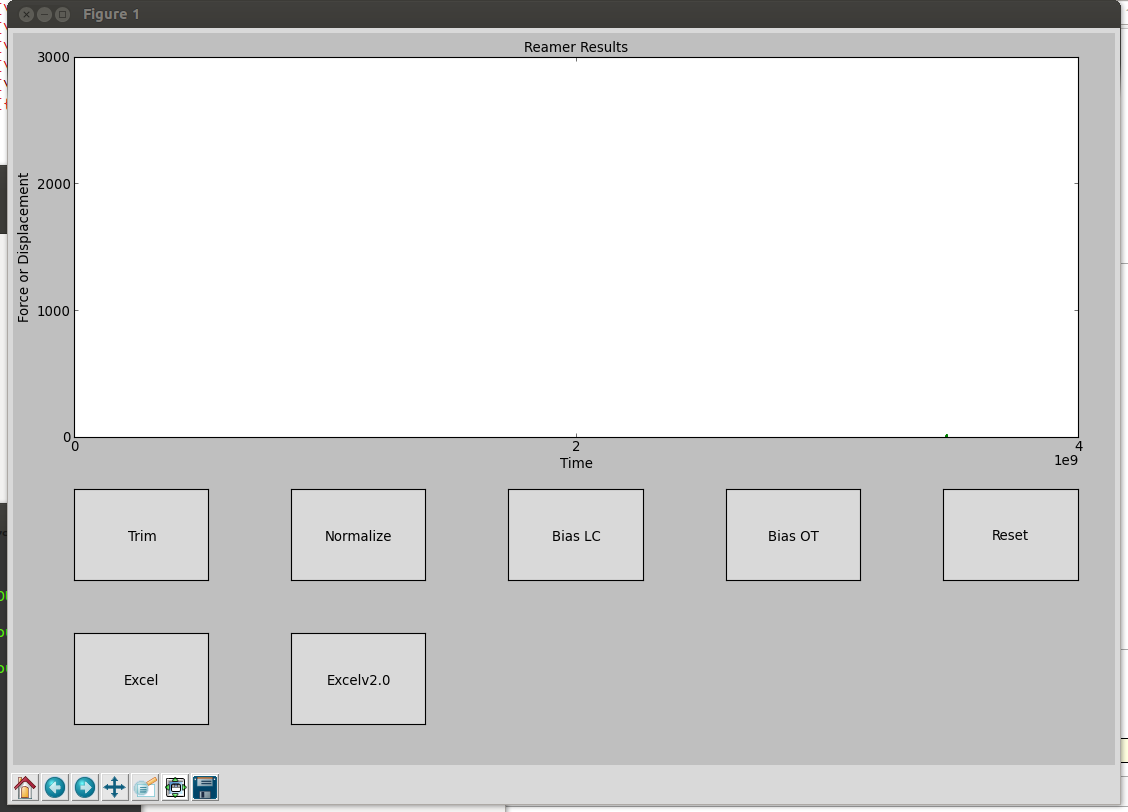
\includegraphics[width=110mm]{./images/gui}
\caption{GUI}
\end{figure}


Now it may appear as if its not working however you need to remember that most of the original timestamp values are ~3,000,000,000. Therefore if we ever expect to see anything meaningful we need to normalize. Show below is an example of what the data looks like normalized. \\

\begin{figure}[ht!]
\centering
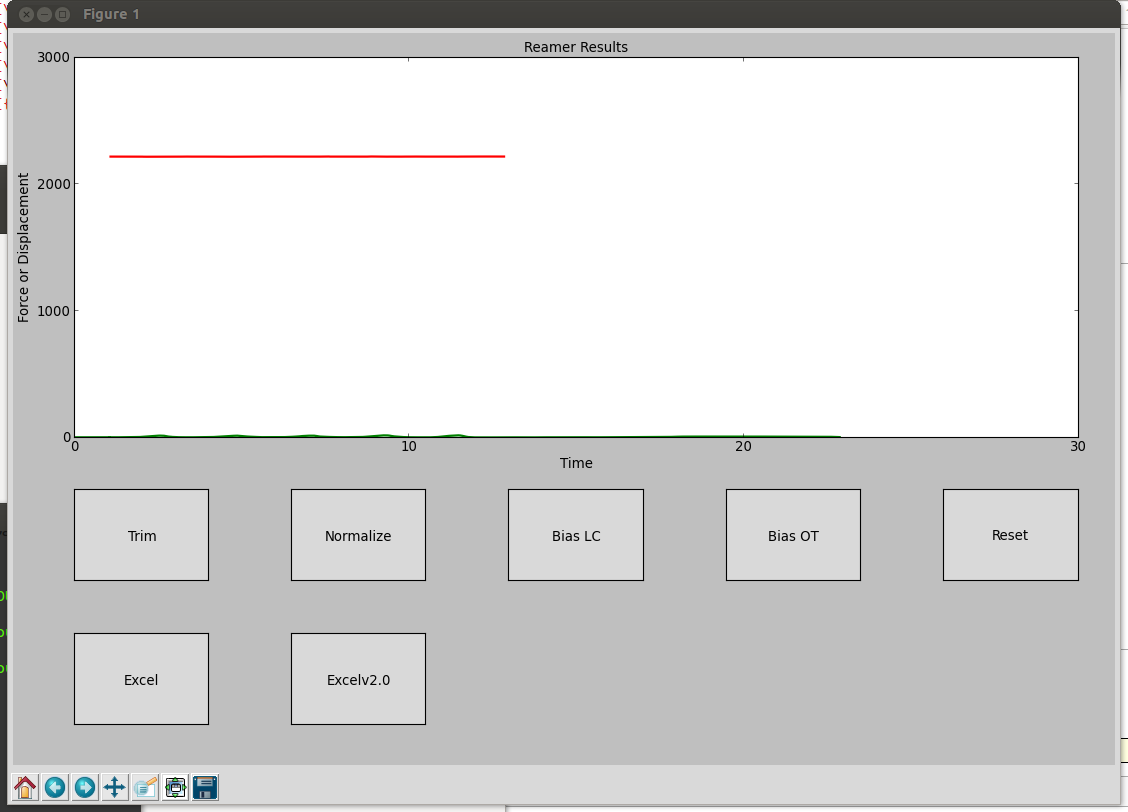
\includegraphics[width=110mm]{./images/gui2}
\caption{GUI Normalized}
\end{figure}

\pagebreak
Next, let's bias both the load cell and optical tracker as shown below. \\

\begin{figure}[ht!]
\centering
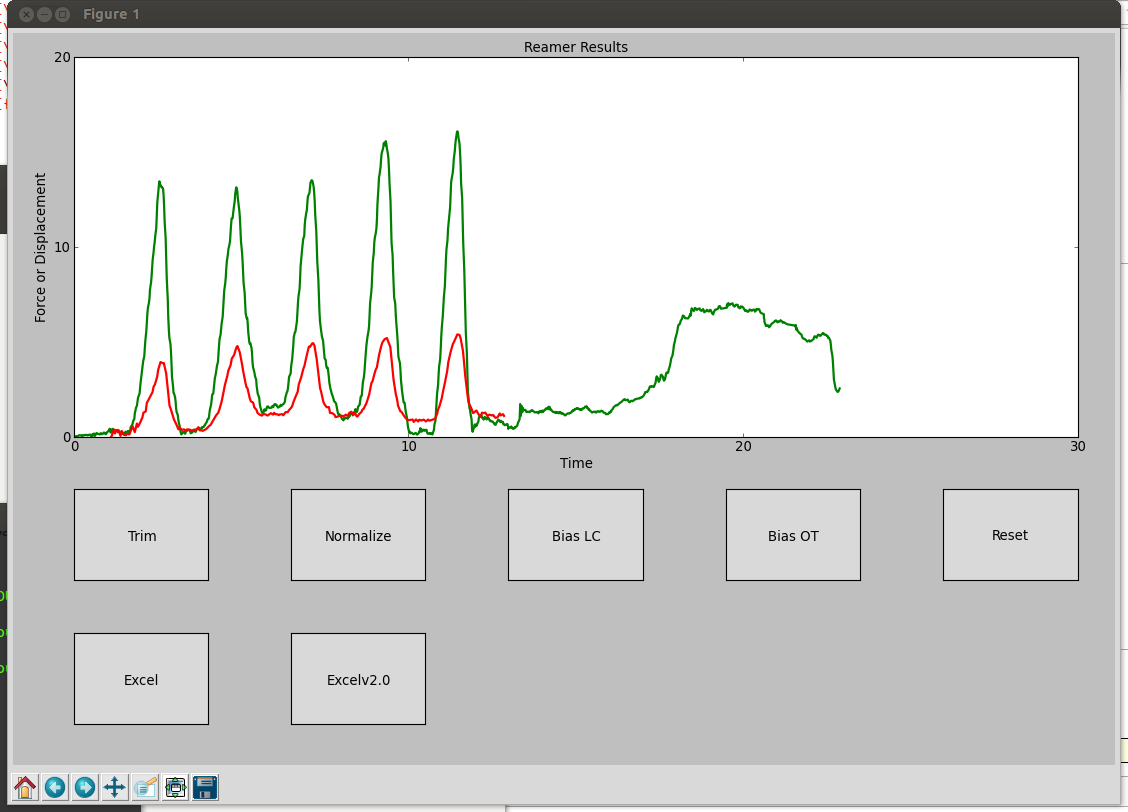
\includegraphics[width=110mm]{./images/gui3}
\caption{GUI Normalized and Biased}
\end{figure}

Now this is starting to look like real data! We can remove the secions at the start and end where we have load cell values without optical tracker by clicking the \textit{Trim} button. \\

\begin{figure}[ht!]
\centering
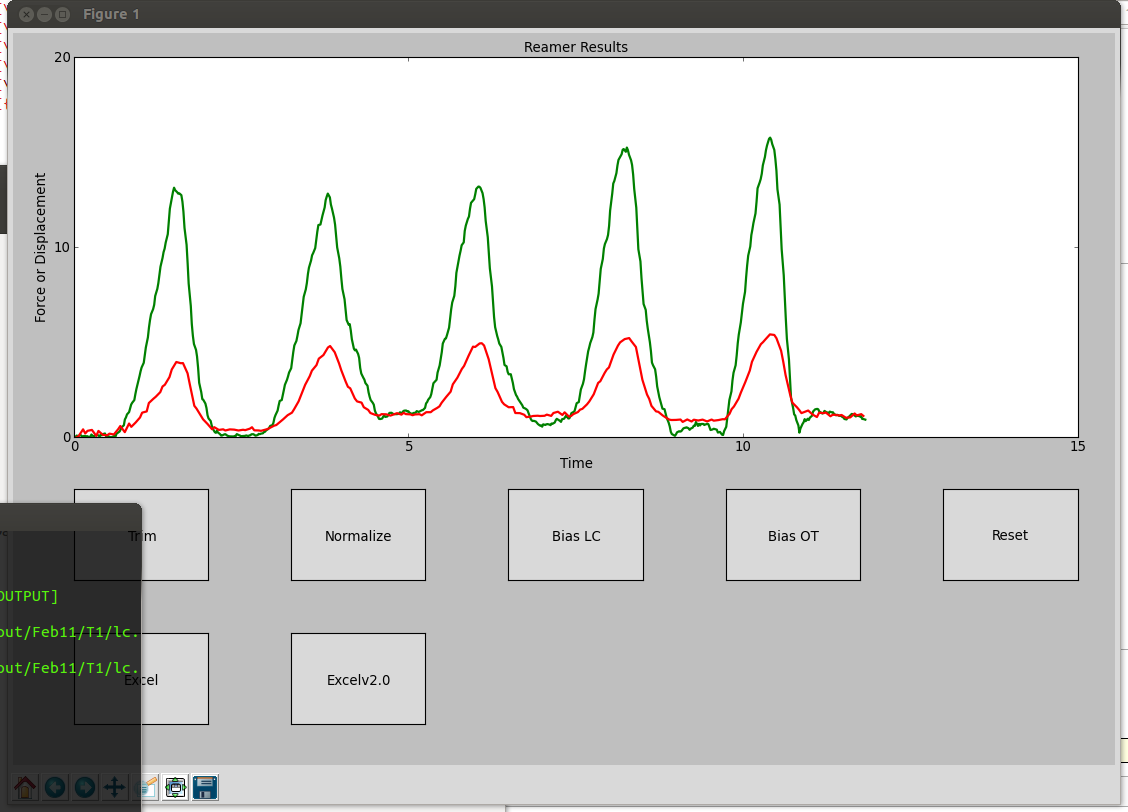
\includegraphics[width=110mm]{./images/gui4}
\caption{GUI Normalized, Biased, and Trimmed}
\end{figure}

Intuitively reset will reset back before we preformed any operations. The last thing to touch on are these Excel and Excelv2.0 buttons. Excel will output the data to the output file specified in the origional command. We have added some very nice functionality where we will interpolate all missing values to give each load cell and optical tracker measurements a complementary pair. This allows us to calculate stiffness and through interpolation richen our data. \\

We will export to excel in the following format:

\begin{table}[h!]
\begin{center}
    \begin{tabular}{ | l | l | l | l |}
    \hline
    Timestamp & Fr & Dr & K \\ \hline
	\end{tabular}
	\caption{Excel}
\end{center}
\end{table}

The excel2.0 button will also remove all values with a Fr below 2.0N. These values can be associated with down time prepping between pushes. This allows us to quickly visually note distincly different pushes. \\

All code will be included in Appendix B. 

\pagebreak
\begin{appendices}
\section{Supplementary Software Files}
\subsection{smart\_02}
\lstinputlisting{./smart_02.rig}
\pagebreak
\subsection{bsty0213.rig}
\lstinputlisting{./bsty0213.rig}
\pagebreak
\subsection{FT13036Nano25ReCalibrated.cal}
\lstset{language=XML}
\lstinputlisting{./FT13036Nano25ReCalibrated.cal}
\lstset{language=Python}
\section{Code}

\subsection{Packets}

\subsubsection{Packet.py}
\lstset{language=Python}
\lstinputlisting{../Packet.py}
\pagebreak

\subsubsection{OpticalTrackerData.py}
\lstset{language=Python}
\lstinputlisting{../OpticalTrackerData.py}
\pagebreak

\subsubsection{LoadCellData.py}
\lstset{language=Python}
\lstinputlisting{../LoadCellData.py}
\pagebreak

\subsection{Sensors}

\subsubsection{Sensor.py}
\lstset{language=Python}
\lstinputlisting{../Sensor.py}
\pagebreak

\subsubsection{LoadCell.py}
\lstset{language=Python}
\lstinputlisting{../LoadCell.py}
\pagebreak

\subsubsection{OpticalTracker.py}
\lstset{language=Python}
\lstinputlisting{../OpticalTracker.py}
\pagebreak


\subsection{Visitor Design Pattern}

\subsubsection{Reamer.py}
\lstset{language=Python}
\lstinputlisting{../Reamer.py}
\pagebreak

\subsubsection{DataExchange.py}
\lstset{language=Python}
\lstinputlisting{../DataExchange.py}
\pagebreak

\subsubsection{Chart.py}
\lstset{language=Python}
\lstinputlisting{../Chart.py}
\pagebreak

\subsubsection{StiffnessElement.py}
\lstset{language=Python}
\lstinputlisting{../StiffnessElement.py}
\pagebreak

\subsection{GUI}

\subsubsection{gui.py}
\lstset{language=Python}
\lstinputlisting{../gui.py}
\pagebreak

\subsubsection{main\_gui.py}
\lstset{language=Python}
\lstinputlisting{../main_gui.py}
\pagebreak


\end{appendices}
\pagebreak
\end{document}
